\documentclass{article}
\usepackage{amsmath}
\usepackage{amssymb}
\usepackage{graphicx}
%\usepackage{enumitem}
\usepackage[utf8]{inputenc}
\graphicspath{{../Imagenes/}}

\title{\Huge Taller de Herramientas Computacionales}
\author{Elías Jiménez Cruz}
\date{15/enero/2019}

\begin{document}
	\maketitle
	\begin{center}
		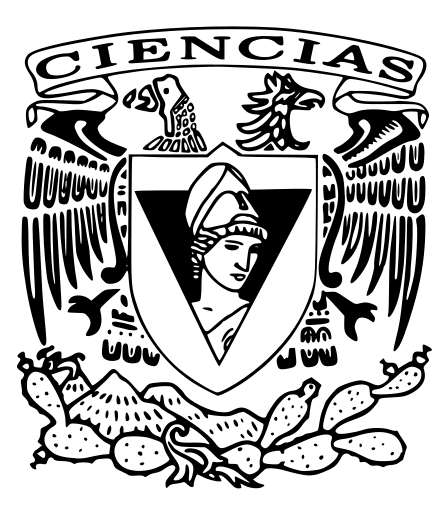
\includegraphics[scale=0.40]{EscudoFC.png}
	\end{center}
	\newpage
	\section*{Expresiones Matemáticas} %Sin asterisco se enumeran las secciones
	$\alpha + \beta$ \\
	\(\alpha +\beta\) \\
	\[\alpha + \beta\]
	\section*{Índices y subíndices}
	$x {2}$
	$x^{2}$
	\section*{Fracciones}
	$\frac{\frac{3}{5}}{2}$, 
	$\sqrt{2} + \sqrt{3^2}^2$, 
	\%, %Para mostrar el porcentaje.
	$\int_{a}^{b} x^2 dx$, 
	$\int_{a}^{b} x^2 \partial x^2$\\
	\begin{equation}
		\label{key}
	\end{equation}
	$3 \quad 2$
\end{document}